\section*{Introduction}

Modern enterprises run cloud applications that span multiple layers, including application logic, container runtimes, and cloud services, creating complex attack surfaces. Adversaries increasingly chain exploits across these layers, yet existing defenses remain fragmented. Cloud-Native Application Protection Platforms (CNAPPs)~\cite{wiz_cdr,orca_cnapp} focus on configuration and posture management but offer little visibility into live application behavior. Host-based EDRs~\cite{crowdstrike} flag isolated process anomalies without cloud context, and cloud-native tools~\cite{aws_guardduty,aws_cdr,paloalto_cdr} detect suspicious API activity without linking it to application or host-level causes. This siloed monitoring leaves security teams blind to the full narrative of multi-stage attacks and forces them to manually correlate disconnected alerts, often too late to prevent damage.

\begin{wrapfigure}{R}{.40\linewidth}
    \centering 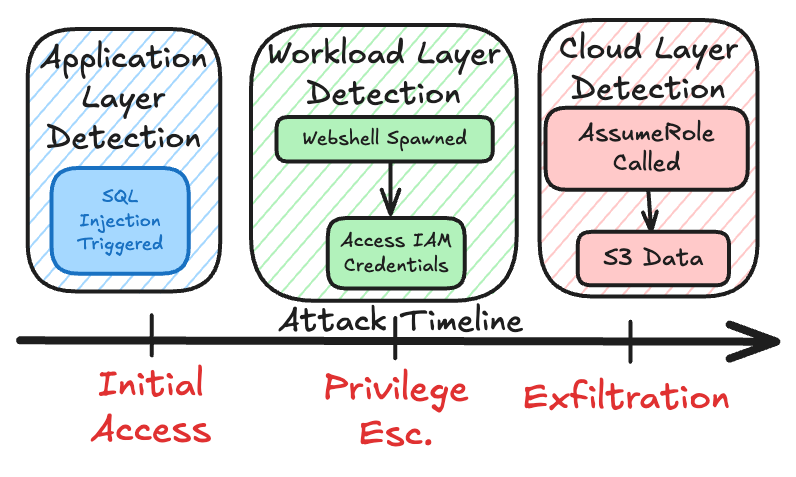
\includegraphics[width=0.40\textwidth]{fig/moveit.png}
    \caption{Timeline of the MOVEit attack highlighting the need for cross-layer visibility across application, workload, and cloud layers for complete detection and investigation.}
    \label{fig:example:moveit}
    \vspace{-2ex}
\end{wrapfigure}

Cloud Application Detection and Response (CADR) offers a necessary shift by unifying observability across application, workload, and cloud layers. Existing cloud detection systems centralize logs for analysis but struggle with correlating events across stack boundaries. This limitation stems from a deeper architectural gap: {\it lack of runtime provenance}. CNAPPs lack execution context, EDRs ignore cloud identities, and cloud-native tools miss process lineage. Without end-to-end causal visibility, advanced threats remain undetected or poorly explained~\cite{omegalog,dossier}.



The MOVEit breach~\cite{progress_moveit_cve2023}, depicted in Figure~\ref{fig:example:moveit}, demonstrates the operational urgency for this shift. A SQL injection at the application layer triggered remote shell access in the workload layer, followed by unauthorized cloud data access through inherited IAM credentials. Each stage of the attack occurred in a different operational plane, but existing tools failed to observe or correlate the entire chain in real time. Even when alerts were raised, they lacked causality, context, and triage guidance. Some tools will flag isolated symptoms, such as anomalous file access or role assumption, but none supported cross-layer reasoning. Incidents like Log4Shell~\cite{cisa_log4j} and Spring4Shell~\cite{intruder_spring4shell} followed similar trajectories from initial injection to lateral host movement and eventual cloud compromise. Without unified telemetry and causally linked reasoning, security teams are left chasing fragments rather than coherent attack narratives.


To address these gaps, we introduce the novel notion of Provenance-based Cloud Application Detection and Response (P-CADR). P-CADR extends provenance principles to the runtime cloud stack by constructing {\it Cross-Layer Provenance Graphs (CPGs)}. These graphs unify semantically rich telemetry from the application, container, and cloud layers, enabling causal reasoning across traditionally disjoint components. This design provides full-stack observability and traceability, allowing security teams to trace attack causality end-to-end. Unlike traditional systems that detect isolated anomalies, P-CADR infers attack narratives by encoding {\it how}, {\it where}, and {\it why} an event occurred in its broader context. It empowers security teams with actionable, explainable incident graphs and enables autonomous response actions mapped to cloud-native APIs. We design algorithms and architectures to leverage CPGs for detecting complex threats and responding in real time, effectively augmenting the transparency of cloud systems and enabling security teams to see the full story of an intrusion, not just isolated fragments.

We propose a three-pronged approach. First, we will develop a cloud-native instrumentation layer using eBPF to collect semantically rich telemetry across all layers (Task~\ref{task:1}). Second, we will construct unified Cross-Layer Provenance Graphs (CPGs) that encode causal interactions using entity linkage, temporal correlation, and semantic motifs (Task~\ref{task:2}). Third, we will develop a provenance-graph-based detection and response engine capable of recognizing complex attack chains (Task~\ref{task:3}).


% \begin{wrapfigure}{L}{.40\linewidth}
\begin{figure}[t!]
    \centering 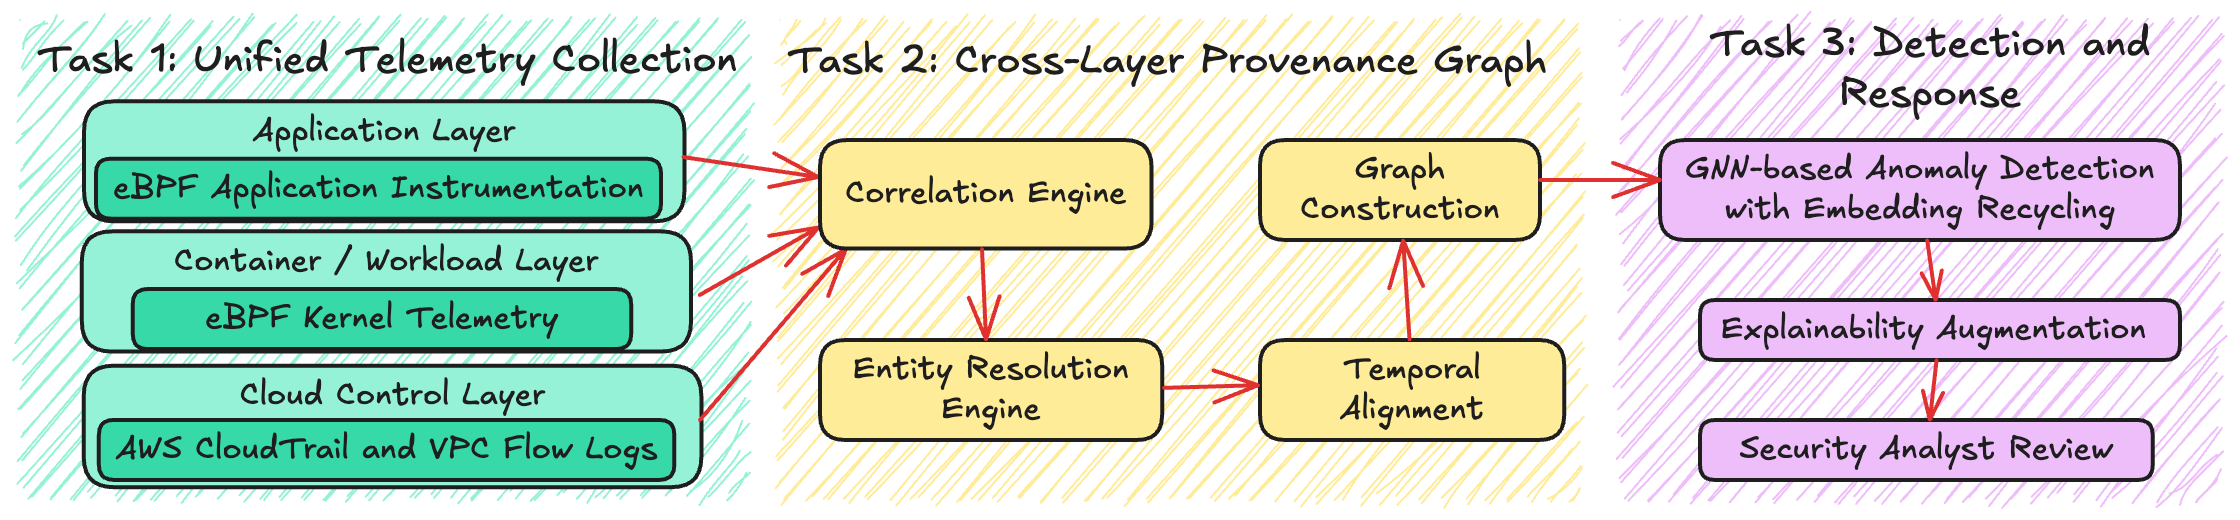
\includegraphics[width=0.90\textwidth]{fig/arch.png}
    \caption{End-to-end workflow showing our three interconnected tasks.}
    \label{fig:arch}
    \end{figure}
% \end{wrapfigure}



\section*{Methods}

\Task{Cross-Layer Runtime Observability Using eBPF}{task:1} Modern attacks often traverse application, workload, and cloud control layers, yet existing security agents remain blind to these multi-layered threat paths. They suffer from poor coverage of interpreted runtimes, lack correlation with cloud APIs, and incur high overhead, especially in containerized, ephemeral environments. We will address these limitations by building a unified observability layer that captures and correlates security-relevant events across all layers.

\begin{wrapfigure}{R}{.30\linewidth}
    \centering 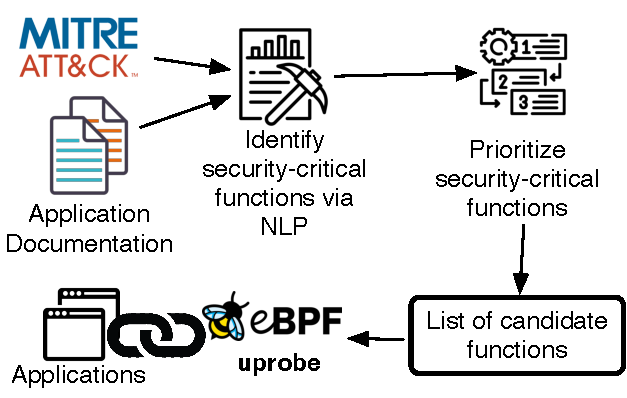
\includegraphics[width=0.30\textwidth]{fig/uprobe-chain.pdf}
    \caption{Workflow for identifying and instrumenting security-critical application functions using NLP-guided analysis and eBPF uprobes.}
    \label{fig:example:uprobe}
    \vspace{-2ex}
\end{wrapfigure}

Our architecture will leverage \textbf{eBPF as a programmable, low-overhead instrumentation substrate}, enabling dynamic tracing of both user-space and kernel-space activity. As shown in Figure~\ref{fig:example:uprobe}, we will develop a workflow that identifies and prioritizes security-critical application functions using NLP over MITRE ATT\&CK and documentation sources. We will then attach \textit{uprobes} to the selected functions for tracing high-level application behavior (e.g., query evaluation, template rendering). In parallel, \textit{kprobes} will monitor low-level system calls (e.g., \CodeIn{execve}, \CodeIn{connect}), and cloud API modules will collect telemetry from CloudTrail, STS, VPC Flow Logs, and Kubernetes audit trails. Each event will be enriched with container metadata (e.g., cgroup, pod, namespace), execution context (PID, UID, IAM identity), and correlation tags, then joined in-kernel using extended BPF maps to minimize overhead and preserve temporal causality.

In the MOVEit breach scenario, our system would capture the SQL injection through an application-layer uprobe, trace the shell spawn via \CodeIn{execve}, monitor IAM escalation through STS logs, and record S3 exfiltration, all causally linked in a unified telemetry graph. We will deploy our instrumentation across AWS EKS clusters, simulate multi-stage attacks using Caldera~\cite{caldera} and Atomic Red Team~\cite{atomicredteam}, and evaluate trace completeness, data fidelity, and CPU/I/O overhead.




\Task{Cross-Layer Provenance Graph Construction (CPG)}{task:2} While Task~1 will enable telemetry collection across application, kernel, and cloud layers, raw logs alone remain insufficient for attack attribution. The key challenge is correlation: identities diverge across layers (e.g., IAM roles vs containers), timestamps are often misaligned, and ephemeral processes or containers lack persistent identifiers. Existing provenance models cannot unify these fragmented signals, nor can they tie host-side activity to cloud-side consequences. Without precise correlation, defenders are left with disconnected clues and incomplete attack narratives.

We will address this by constructing real-time Cross-Layer Provenance Graphs (CPGs) that fuse heterogeneous telemetry into a single causal structure. To solve the correlation problem, we will use application-layer hooks to intercept AWS SDK calls, logging explicit links between processes and cloud API actions. For unhooked events, we will apply time-and-entity correlation, matching processes that initiate connections to cloud endpoints with subsequent CloudTrail events, augmented by cloud metadata such as instance IDs and request IDs. IAM roles will be represented as nodes, and privilege transitions via AssumeRole will form causal edges connecting roles, API calls, and originating processes. We will resolve identity mismatches using metadata fingerprinting, fuzzy role matching, and container ancestry tracking~\cite{huo2023semparser,le2023log,nawaz2021fuzzy}. Temporal misalignment will be addressed with adaptive windowing~\cite{bifet2007learning} and entropy-based alignment~\cite{makanju2010evaluation}.

Figure~\ref{fig:example:cpg} illustrates how the MOVEit attack will be captured end-to-end, linking SQL injection, shell spawn, credential access, IAM role usage, and S3 exfiltration in a unified graph. This graph structure enables precise investigation and forms the basis for Task~3, where we will apply graph-based deep learning techniques to detect anomalous paths and unseen attack patterns. We will evaluate CPGs based on fidelity against expert-labeled traces, ingestion latency under burst load, and memory overhead in continuous deployment.

\begin{figure}[t!]
    \centering 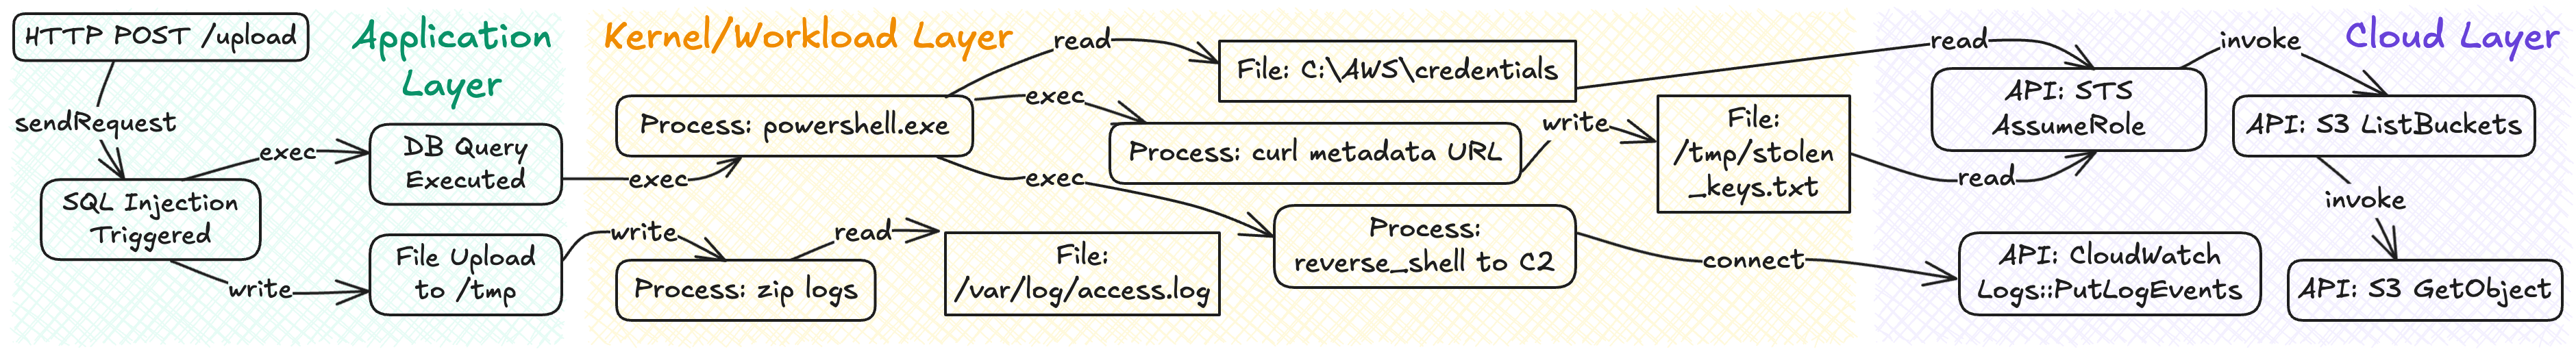
\includegraphics[width=0.99\textwidth]{fig/graph-example.png}
    \caption{Example Cross-Layer Provenance Graph (CPG) for the MOVEit attack scenario.}
    \label{fig:example:cpg}
\end{figure}

\Task{Provenance-Guided Detection and Automated Response}{task:3} The CPGs constructed in Task~\ref{task:2} will serve as the foundation for this downstream threat detection task. Traditional tools lack the ability to trace fine-grained, multi-step attack chains and often miss stealthy tactics that span across system and cloud layers. They rely on static signatures or coarse anomaly metrics, producing noisy alerts with limited context. By leveraging rich, real-time CPGs, we can detect complex adversarial behaviors with greater precision, explainability, and coverage.

We will build a detection engine that processes streaming subgraphs from CPGs using a hybrid learning pipeline. We will extract candidate subgraphs using sliding windows and model them using supervised GNN classifiers, such as GraphSAGE~\cite{lo2022graphsage} and GAT~\cite{velivckovic2017graph} to assign semantic labels. PI Hassan’s prior system, Flash~\cite{flash2024}, successfully detected APTs on single-host provenance graphs; here, we will extend that methodology to multi-layer CPGs. To accelerate inference, we will incorporate embedding recycling, a technique introduced in Flash~\cite{flash2024}, to avoid recomputing node embeddings for stable regions of the graph. To improve analyst trust and enable human-in-the-loop validation, we will adapt GNNExplainer~\cite{ying2019gnnexplainer} and PGExplainer~\cite{luo2020parameterized} to generate subgraph-level justifications that highlight the key entities and transitions responsible for triggering an alert. We will evaluate detection performance using traces from MOVEit, XZ Utils, Spring4Shell, and custom APT simulations. Metrics will include detection precision, false positive rate, response latency, and accuracy in triage tasks.

\section*{Expected results}
We will release instrumentation code and cross-layer telemetry datasets by Month 3, complete the CPG construction engine by Month 6, deliver the detection and explanation modules with code and benchmarks by Month 9, and submit a peer-reviewed publication and present results by Month 12. Technical reports and documentation will be shared throughout.
    
\section*{Funds Needed}

We request \$60,000 for one year of graduate student support (stipend, tuition, health insurance) and \$15,000 for one month of summer salary for PI Hassan. Additionally, we seek \$25,000 in AWS Promotional Credits to support ML workloads and data storage. Our experiments on p3.2xlarge and m5.large instances will support ML training and baseline system operations. We also require 3 TB of secure Amazon S3 storage for Task~\ref{task:1} logs. The credits will cover these expenses.

